\documentclass[letterpaper,11pt,openany]{book}
\usepackage{knowledge}

\title{Элементы криптографического анализа}
\author{Автор курса: Тимонина Елена Евгеньевна \\ 
		Составитель: Смирнов Дмитрий Константинович }
\date{Версия от \currenttime, \today}

\begin{document}

\maketitle
\tableofcontents

\mainmatter

\chapter{Домашние задания}

\section{Введение}

\section{Определение шифра. Простейшие примеры.}

\task{Что такое подстановка?}
Подстановка — это взаимно однозначная функция, которая переводит буквы алфавита в буквы того же самого алфавита.

\task{Что такое группа, и почему множество $S_m$ из примера 2.1 образует группу?}
Множество $G \ne \varnothing$ с бинарной операцией $"\circ"$, называется \emph{группой}, если выполнены условия:

1. $ \forall a,b \in G \;\; a \circ b \in G; $

2. $ \forall a,b,c \in G \;\; a \circ (b \circ c) = (a \circ b) \circ c; $

3. $ \exists e \in G \colon \forall a \in G \;\; e \circ a = a \circ e = a;$

4. $ \forall a \in G \;\; \exists b \in G \colon a \circ b = b \circ a = e$

Множество $S_m$ вводится как множество всех подстановок на конечном алфавите $A = \{a_1, ... , a_m\} $. Проверим выполнение аксиом группы:

1. Подстановка $k \in S_m$ -- отображение $k \colon A \to A$. $\forall k_1, k_2 \in S_m $ рассмотрим суперпозицию $k_1 \circ k_2$. Так как $k_1 \circ k_2 \colon A \to A \to A$, то $k_1 \circ k_2 \in S_m $ и первая аксиома верна.

2. $\forall k_1, k_2, k_3 \in S_m \;\; k_1 \circ (k_2 \circ k_3) = k_1 \circ k_2 ( k_3 (a)) = k_1 ( k_2 ( k_3 (a))) = k_1 ( k_2 (a)) \circ k_3 (a) = (k_1 \circ k_2) \circ k_3$.

3. Поскольку $S_m$ -- множество всех подстановок, то найдётся тождественная подстановка: $\exists e \in S_m \colon \forall a \in A \;\; e(a) = a$. Тогда $\forall k \in S_m $ верно $e \circ k = e(k(a)) = k(a) = k(e(a)) = k \circ e$.

4. Так как подстановка -- взаимно однозначная функция, то $\forall k \in S_m $ существует обратная функция: $\exists k^{-1} \colon A \to A \Rightarrow k^{-1} \in S_m$, для которой будет выполнено равенство $k \circ k^{-1} = k (k^{-1}(a)) = k^{-1} (k(a)) = k^{-1} \circ k$. При этом, $\forall a \in A \;\; k^{-1} (k(a)) = a = e(a)$.

Выполнены все аксиомы группы, следовательно $S_m$ -- группа.

\task{Почему группа $S_n$ из примера 2.2 является симметрической?}
Симметрической группой $n$-го порядка называется множество S(X) всех биективных отображений $f \colon X \to X$, где $X$ -- конечное множество из n элементов.
Группа $S_n$ в примере 2.2 определяется как группа подстановок на множестве $X = \{1,...,n\}$. Подстановка -- это биективное отображение, X -- конечное множество из n элементов. Следовательно, по определению, группа $S_n$ является симметрической.

\task{Что такое кольцо? Что такое кольцо вычетов по модулю $m$?}
Множество $K$ называется \emph{кольцом}, если в $K$ определены две операции $"+"$ (сложение) и $"\cdot"$ (умножение) и выполняются следующие условия $\forall a, b, c \in K$:

1. $a + b \in K, a \cdot b \in K$;

2. $a+(b+c) = (a+b)+c, \; a(bc) = (ab)c$;

3. $a+b = b+a$;

4. $(a+b)c = ac+bc$;

5. $\exists 0 \in K \colon a + 0 = a$.

Кольцом вычетов по модулю $m$ называется такое кольцо \\ $\mathbb{Z}_{/m} = \{C_0, C_1, ..., C_{m-1}\}$ ($C_r$ -- смежный класс вычетов по модулю $m$), в котором операции сложения и умножения определяются следующими правилами:

1. $C_a + C_b = C_r$, \; где $r \equiv (a+b)(\!\!\!\!\mod m)$;

2. $C_a C_b = C_r$, \; где $r \equiv ab(\!\!\!\!\mod m)$

То есть, $C_a + C_b$ -- это класс, в который входит число $a+b$, а $C_a C_b$ -- класс, в который входит число $ab$.

\task{Какую алгебраическую структуру представляет собой кольцо $\mathbb{Z}_{/m}$ при $m = 2$?}

\begin{theorem}
\label{ring_is_field}
Если $p$ -- простое число и $p \ge 2$, то $\mathbb{Z}_{/m}$ -- поле характеристики $p$.
\end{theorem}

По теореме \ref{ring_is_field} кольцо $\mathbb{Z}_{/2}$ является полем характеристики 2.


\section{Стойкость шифров. Метод полного перебора.}

\task{Дан алфавит $A = \{1,2,...,n\}$, $x$ -- открытый текст в алфавите $A$. Ключ шифрования $(T_1, T_2, T_3)$, где $T_i$ -- случайные подстановки. Алгоритм шифрования: $T_3(T_2(T_1(x))) = y$. Какова формула для расшифрования? Мощность пространства различных ключей? Сложность МПП?}

1. Формула для расшифрования -- $x = T_1^{-1}(T_2^{-1}(T_3^{-1}(y))).$

2. В каждой подстановке на первое место можно поставить $n$ различных букв, на второе -- $n - 1$, и т.д. В итоге получаем $n!$ вариантов на каждую подстановку, следовательно, $|K| = (n!)^3$ для трёх подстановок.

3. Пусть в тексте $a$ букв. Тогда необходимо провести $3a$ операций подстановки, чтобы проверить один ключ. В среднем нужно проверить количество ключей, равное средней трудоёмкости МПП: $E\tau = \frac{|K| + 1}{2} = \\ = \frac{(n!)^3 + 1}{2}$. Следовательно, сложность МПП равна $\frac{3}{2}a[(n!)^3 + 1].$

\task{Найти минимальную среднюю трудоёмкость в следующей схеме шифрования:

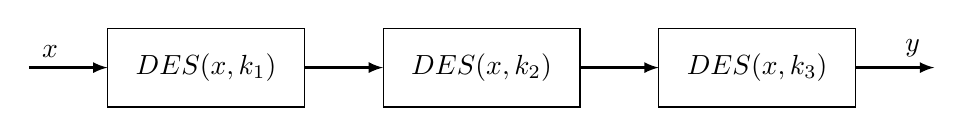
\begin{tikzpicture}[>=latex]
{\centering
\draw[thick, ->] (0,0) -- node[above left] {$x$} (1,0);
\draw (1,-0.5) rectangle node[midway] {$DES(x, k_1)$} (3.5,0.5);
\draw[thick, ->] (3.5,0) -- (4.5,0);
\draw (4.5,-0.5) rectangle node[midway] {$DES(x, k_2)$} (7,0.5);
\draw[thick, ->] (7,0) -- (8,0);
\draw (8,-0.5) rectangle node[midway] {$DES(x, k_3)$} (10.5,0.5);
\draw[thick, ->] (10.5,0) -- node[above right] {$y$} (11.5,0);
}
\end{tikzpicture}

}

В предложенной схеме используется три блока DES с разными ключами. Для одного блока DES $|K| = 2 ^ {56}$, тогда для всей схемы:

\noindent $|K| = (2 ^ {56}) ^ 3 = 2 ^ {168}$. Окончательно, $E\tau = \frac{|K| + 1}{2} = \frac{2 ^ {168} + 1}{2} \approx 2 ^ {167}$.

\task{В сообщении каждая буква записывается два раза. Для шифрования используется шифр перестановки длины $2n$. Сложность МПП?}

В данной схеме используется две подстановки, причём для каждой нечётной буквы применяется первая подстановка, а для каждой чётной~-- вторая: $T(x) = T(x_1, x_2, ... , x_{2l - 1}, x_{2l}) = (T_1(x_1), T_2(x_2), ..., T_1(x_{2l - 1}), T_2(x_{2l}))$, где $l$ -- половина длины сообщения. Тогда длина ключа для каждой из подстановок будет равна $n$, а мощность пространства различных ключей для всей системы будет равна $|K| = (n!)^2$.

Для проверки одного ключа $(T_1, T_2)$ требуется $2l$ операций подстановки. Тогда сложность МПП равна $2lE\tau = 2l\frac{|K| + 1}{2} = l[(2n)! + 1]$.

\task{

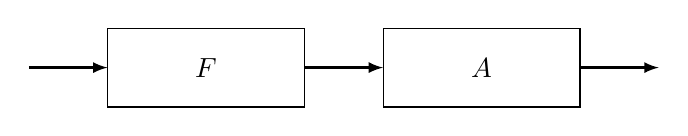
\begin{tikzpicture}[>=latex]
{\centering
\draw[thick, ->] (0,0) -- (1,0);
\draw (1,-0.5) rectangle node[midway] {$F$} (3.5,0.5);
\draw[thick, ->] (3.5,0) -- (4.5,0);
\draw (4.5,-0.5) rectangle node[midway] {$A$} (7,0.5);
\draw[thick, ->] (7,0) -- (8,0);
}
\end{tikzpicture}

В данной схеме байт ОТ $x = x_1 x_2 ... x_8$ шифруется с помощью функции $F$ следующим образом:

$x_1' = x_1$;

$x_2' = x_2 + f_1(x_1)$;

$...$

$x_8' = x_8 + f_8(x_1, x_2, ..., x_7)$,

\noindent где $f_1, ..., f_7$ -- случайные булевы функции, $A$ -- невырожденная матрица. Ключом являются $F$ и $A$. Оценить сложность нахождения ключа с помощью МПП.

}

Определим мощность пространства ключей для $F$. Так как количество функций, зависящих от $n$ переменных, равно $2^{2^n}$, то 
$$|K_F| = \prod_{i = 1} ^ {7} 2^{2^i} = 2 ^ {\sum_{i = 1} ^ {7} 2 ^ i} = 2 ^ { \frac{2(2^7 - 1)}{2 - 1} } = 2 ^ {2^8 - 2} = 2 ^ {254}.$$

Теперь рассмотрим матрицу $A$. Мы на неё умножаем вектор длины~\ 8 и на выходе тоже получаем вектор длины 8. Следовательно, $A \in~\{0,1\}^{8 \times 8}$. Тогда $|K_A| = 2 ^ {8 \cdot 8} = 2 ^ {64}$. Таким образом, 
$$|K| = |K_F| \cdot |K_A| = 2 ^ {254} \cdot 2 ^ {64} = 2 ^ {318}$$

Если бы нам были известны функции $f_1,...,f_7$, то можно было бы рассчитать количество операций на каждый ключ точно. Но нам они неизвестны, поэтому примем за общее число операций для проверки одного ключа за $p$. Тогда сложность МПП равна $\frac{|K| + 1}{2}p = \frac{2^{318} + 1}{2}p \approx 2 ^ {317} p.$ \\

\noindent \textbf{Комментарий к задачам о многочлене Жегалкина.}

В полином Жегалкина степени не выше $m$ от функции $n$ переменных входит $C_n ^ k$ различных мономов степени $k$. При этом перед каждым из них стоит коэффициент, следовательно, $2 ^ {C_n ^ k}$ -- количество различных вариантов выбрать 0 или 1 перед мономами.

Если полином степени ровно $m$, то хотя бы при одном мономе этой степени стоит коэффициент 1. Это означает, что число различных вариантов выбрать 0 или 1 перед мономами степени $m$ в таком полиноме равно $2 ^ {C_n ^ m - 1}$.

Используя полином Жегалкина степени не выше $m$, будем считать, что $n = m$.

\task{Ключ шифрования k -- многочлен Жегалкина степени 2. Мощность пространства различных ключей? Сложность МПП?}

\noindent $|K| = 2 ^ {C_n ^ 0 + C_n ^ 1 + C_n ^ 2 - 1} = 2 ^ {n + \frac{(n-1)n}{2}} = 2 ^ { \frac{n ^ 2 + n}{2} }.$

\noindent Количество операций $p = C_n ^ 1 (1 + 1) + C_n ^ 2 (1 + 2) = 2n + 3 \frac{(n-1)n}{2} = \frac{3}{2} n ^ 2 + \frac{1}{2} n$

\noindent Сложность: $pE\tau = (\frac{3}{2} n ^ 2 + \frac{1}{2} n) \frac{2 ^ { \frac{n ^ 2 + n}{2} } + 1}{2} \approx (3n ^ 2 + n) 2 ^ { \frac{n ^ 2 + n - 4}{2} }$

С учётом последнего комментария получим $|K| = 8$, $pE\tau = 31.5$.

\task{Ключ шифрования k -- многочлен Жегалкина степени не выше $m$. Мощность пространства различных ключей? Сложность МПП?}

\noindent $|K| = 2 ^ { \sum _{i = 0} ^ m C_n ^ i}.$

\noindent Количество операций $p = \sum _{i = 1} ^ m C_n ^ i (i + 1)$

\noindent Сложность: $pE\tau = [\sum _{i = 1} ^ m C_n ^ i (i + 1)] \frac{2 ^ { \sum _{i = 0} ^ m C_n ^ i} + 1}{2} \approx [\sum _{i = 1} ^ m C_n ^ i (i + 1)] 2 ^ { \sum _{i = 1} ^ m C_n ^ i}$

\task{Ключ шифрования k -- многочлен вида:
$$\sum_{1 \le i < j \le n } a_{ij} x_i x_j, a_{ij} \in \{0, 1\}.$$
Мощность пространства различных ключей? Сложность МПП?}

Множество $a_{ij}$ образует верхнетреугольную матрицу без главной диагонали. Следовательно, $|K| = 2 ^ {(n - 1) + (n - 2) + ... + 1 + 0} = 2 ^ { \frac{(n-1)n}{2} }$.

\noindent Количество операций $p = \frac{(n-1)n}{2}(1 + 2) - 1 = \frac{3}{2} n ^ 2 - \frac{3}{2} n - 1$

\noindent Сложность: $pE\tau = (\frac{3}{2} n ^ 2 - \frac{3}{2} n - 1) \frac{2 ^ { \frac{(n-1)n}{2} } + 1}{2} \approx (3 n ^ 2 - 3 n - 2) 2 ^ { \frac{n ^ 2 - n - 4}{2}}$

\end{document} 
